\documentclass[10pt, a4paper]{article}
% \documentclass[10pt, a4paper]{ctexart}
\usepackage[left=3.17cm, right=3.17cm, top=2.54cm, bottom=2.54cm]{geometry}
\usepackage[numbers,sort&compress]{natbib}
\renewcommand\refname{参考文献}
\newcommand{\upcite}[1]{\textsuperscript{\textsuperscript{\cite{#1}}}}
\usepackage{caption}
\usepackage{multirow}
\usepackage{appendix}
\usepackage{graphicx, subfigure}
\usepackage[UTF8]{ctex}
\usepackage{amssymb,amsmath}
\usepackage{pgf,tikz,pgfplots}
\pgfplotsset{compat=1.15}
\usepackage{mathrsfs}
\usepackage{listings}
\usepackage{booktabs}
\usetikzlibrary{arrows}
\setmainfont{Source Serif Pro}
\setsansfont{Source Sans Pro}
\setmonofont{Source Code Pro}

\lstset{
 columns=fixed,   
 breaklines,
 frame=none,                                          % 不显示背景边框
 basicstyle=\small,
 backgroundcolor=\color[RGB]{245,245,245},            % 设定背景颜色
 keywordstyle=\color[RGB]{40,40,255},                 % 设定关键字颜色
 numberstyle=\footnotesize\color{darkgray},           
 commentstyle=\it\color[RGB]{0,96,96},                % 设置代码注释的格式
 stringstyle=\rmfamily\slshape\color[RGB]{128,0,0},   % 设置字符串格式
 showstringspaces=false,                              % 不显示字符串中的空格
 language=matlab,                                        % 设置语言
}

\begin{document}

\title{数字信号处理第二次课程设计报告\\\textbf{DTMF信号的检测与识别}}
%\author{无86\quad 沈逸昕\quad 2018011209}
\author{BobAnkh}

\maketitle

\section{算法原理和设计思路}

\subsection{DTMF信号产生}

    DTMF信号可直接利用行频和列频两组正弦信号的叠加来产生。行频和列频分别包含4个频率,每个按键对应着一个行频和列频的频率组合,因此DTMF信号共有16个编码。DTMF信号的具体频率配置见下图:
    
    \centerline{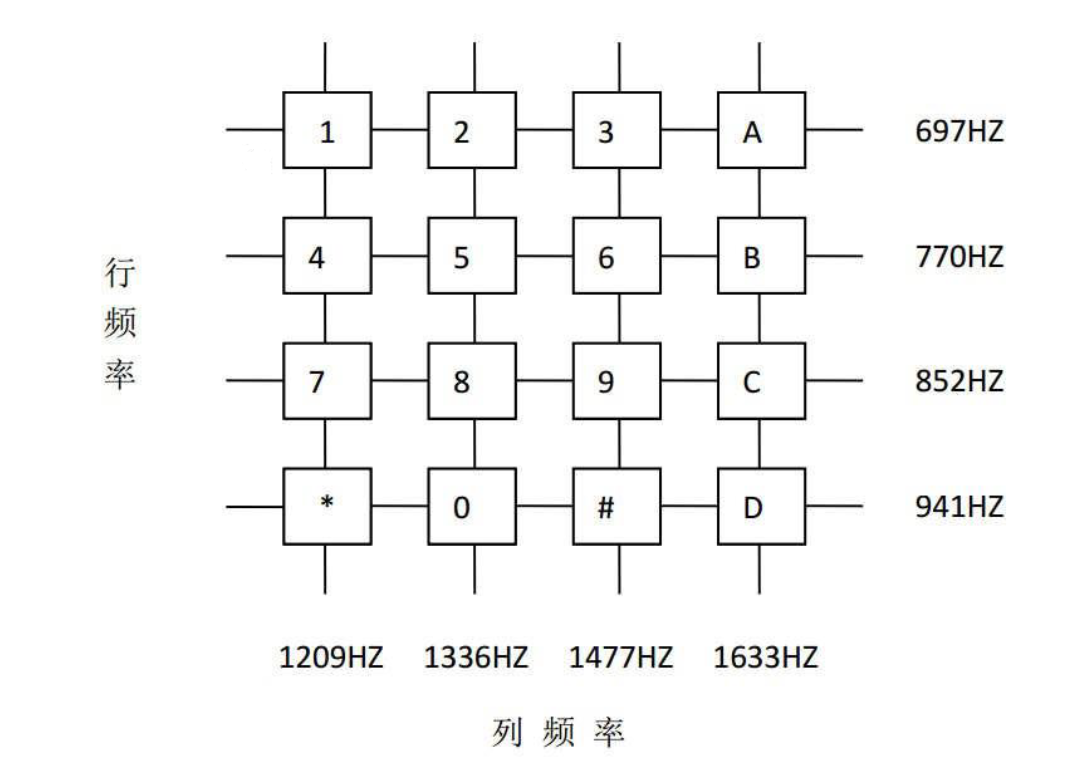
\includegraphics[scale=0.4]{assets/1.png}}
    
    根据如下差分公式和框图设计数字正弦振荡器,进行正弦信号的产生,进而编写DTMF信号产生程序——根据读取到的键值查表得到对应的双频,从而产生对应的DTMF信号。\\
    
    
    差分方程:
    $$
    \left\{ 
    \begin{array}{c}
        y_c[n]=(cos\omega_0)y_c[n-1]-(sin\omega_0)y_s[n-1] \\  y_s[n]=(sin\omega_0)y_c[n-1]+(cos\omega_0)y_s[n-1] \\
    \end{array}
    \right. 
    $$
    
    起始条件:
    $$
    \left\{ 
    \begin{array}{c}
        y_c[-1]=cos\omega_0 \\ y_s[-1]=-sin\omega_0 
    \end{array}
    \right. 
    $$
    
    框图:
    
    \centerline{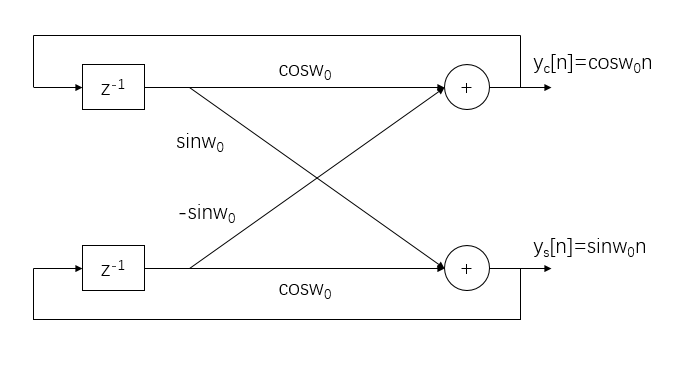
\includegraphics[scale=0.6]{assets/2.png}}

\subsection{DTMF信号检测与识别}

\subsubsection{采用FFT方法来进行检测识别}

    利用FFT直接计算输入信号的DFT,通过对信号整个频域信息的分析来检测DTMF的存在并识别相应的按键。
    
    具体实现中,根据时域信号确定合适的FFT点数后采用FFT得到频谱,在可能的频率范围内,使用Matlab自带的\texttt{findpeaks}函数寻找峰值,找出两个最大的峰值并确定其对应的频率,根据频率查表来判别对应的按键值,部分参数的选取也是实际尝试之后得到。对于频率查表也采用了20Hz的误差容限。
    
    编写了如下的\texttt{find\_key\_fft}函数来进行检测,接受时域信号序列和采样率,返回按键值key,相关代码如下:

    \begin{lstlisting}
    function key = find_key_fft(xn, fs)
    %find_key_fft: 使用fft来寻找键值
    %   xn: 待测音频序列
    %   fs: 采样率
        keys = [
        '1', '2', '3', 'A';
        '4', '5', '6', 'B';
        '7', '8', '9', 'C';
        '*', '0', '#', 'D'];
        len_x = length(xn);    
        N = 2 ^ nextpow2(len_x);
        X = fft(xn, N);
        X_abs = abs(X(1 : round(2000 / fs * N)));
        [~, locs] = findpeaks(X_abs, 'MinPeakHeight', max(X_abs) * 0.01, 'MinPeakDistance', floor(200 / fs * N), 'SortStr','descend','MinPeakProminence',10);
        if length(locs) < 2
            key = 'X';
        else
            freq1 = (min(locs(1:2)) - 1) / N * fs;
            freq2 = (max(locs(1:2)) - 1) / N * fs;
            if freq1 > 677 && freq1 < 717
                row = 1;
            elseif freq1 > 750 && freq1 < 790
                row = 2;
            elseif freq1 > 832 && freq1 < 872
                row = 3;
            elseif freq1 > 921 && freq1 < 961
                row = 4;
            else
                row = -1;
            end
    
            if freq2 > 1189 && freq2 < 1229
                col = 1;
            elseif freq2 > 1316 && freq2 < 1356
                col = 2;
            elseif freq2 > 1457 && freq2 < 1497
                col = 3;
            elseif freq2 > 1613 && freq2 < 1653
                col = 4;
            else
                col = -1;
            end
            if row == -1 || col == -1
                key = 'X';
            else
                key = keys(row, col);
            end
        end   
    end

    \end{lstlisting}

\subsubsection{采用Goertzel算法来进行检测识别}

    考虑到检测DTMF信号时只关心其8个已知频率的行频/列频信息,故可以有选择地计算特定频率点处的频域信息,以大大降低计算复杂度。Goertzel算法正是利用相位因子的周期性,将DFT计算表示为线性滤波形式,实现了有选择地计算特定频点处频域信息的效果。基于一定的数学推导,可以得到如下的迭代公式:
    \begin{align*}
        v_k[n]&=2cos(\omega_k)v_k[n-1]-v_k[n-2]+x[n] \\
        y_k[n]&=v_k[n]-W_N^k v_k[n-1]
    \end{align*}
    
    具体实现中,按照迭代公式进行运算,取前四位最大值对应的频点为行频,后四位最大值对应的频点为列频,同样查表来判别对应的按键值。
    
    编写了如下的\texttt{find\_key\_goertzel}函数来进行检测,接受时域信号序列和采样率,返回按键值key,相关代码如下:
    
    \begin{lstlisting}
    function key = find_key_goertzel(xn, fs)
    %find_key_goertzel: 使用goertzel来寻找键值
    %   xn: 待测音频序列
    %   fs: 采样率
        freq_list = [697, 770, 852, 941, 1209, 1336, 1477, 1633];
        keys = [
        '1', '2', '3', 'A';
        '4', '5', '6', 'B';
        '7', '8', '9', 'C';
        '*', '0', '#', 'D'];
        N = length(xn);
        omega_list = 2 * pi * round(freq_list / fs * N) / N;
        cos_wk = cos(omega_list);
    
        v0 = zeros(1, 8);
        v1 = zeros(1, 8);
        v = zeros(1, 8);
        for a = 1 : N
            v0 = v1;
            v1 = v;
            v = 2 * cos_wk .* v1 - v0 + xn(a);
        end
        XK = v - v1 .* exp(-1j * omega_list);
        [~, row] = max(abs(XK(1:4)));
        [~, col] = max(abs(XK(5:8)));
        key = keys(row, col);
    end
    \end{lstlisting}

\subsubsection{长音频文件识别}

    在本问中,主要需要实现的是分段的算法。具体的算法思路是:从左到右扫描整段时域音频信号,如果发现目前的值大于某一阈值,则认为这是某一段DTMF信号的起点,此时继续向右扫描;如果发现某一点及其后连续100个点均小于阈值,则标记此时的位置为这一段DTMF信号的终点。保留起点和终点的位置后,重复这样的扫描直至音频信号的末尾。相关代码封装为了一个函数,具体如下:
    
    \begin{lstlisting}
    function [start, finish] = segment(xn)
    % segment: 切分出DTMF信号,返回起点和终点的位置数组
    %   xn: 时域信号
    threshold = 0.1 * max(xn);
    win_len = 100;
    frame = 1;
    
    xn_len = length(xn);
    start = [];
    finish = [];
    silence = true;
    
    while frame <= xn_len
        if xn(frame) > threshold && silence
            start = [start, frame];
            silence = false;
        end
        if sum(xn(frame:min(xn_len, frame + win_len)) > threshold) == 0 && ~silence
            finish = [finish, frame];
            silence = true;
        end
        frame = frame + 1;
    end
    if length(start) - length(finish) == 1
        finish = [finish, xn_len];
    end
    
    end
    \end{lstlisting}

    在有了分段结果之后,将各分段DTMF信号分别取出送入到fft或者goertzel方法中得到按键值,从而可获得长音频中的全部DTMF信号对应的按键值串。

\section{程序流程图}

\subsection{DTMF信号产生}
\centerline{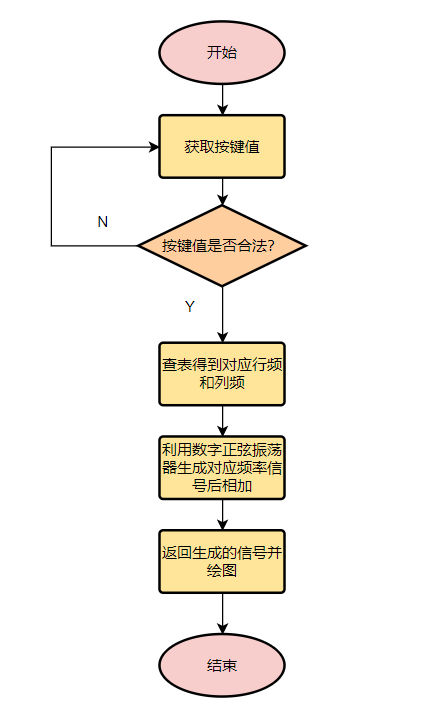
\includegraphics[scale=0.8]{assets/3.png}}

\subsection{DTMF信号检测识别}
左侧为FFT方法,右侧为Goertzel算法

\centerline{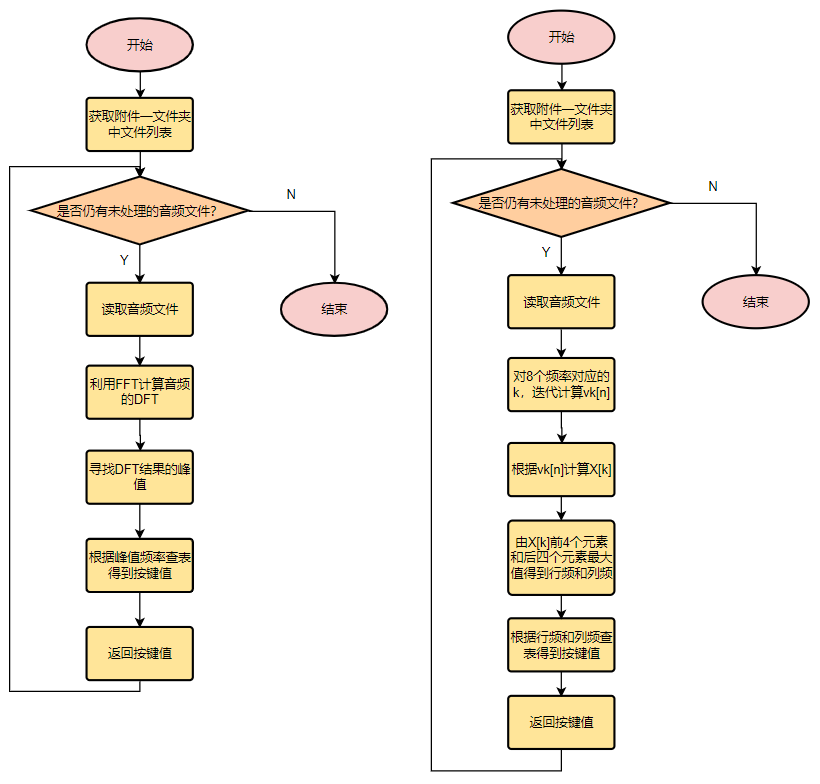
\includegraphics[scale=0.8]{assets/7.png}}

\subsection{长音频检测}
\centerline{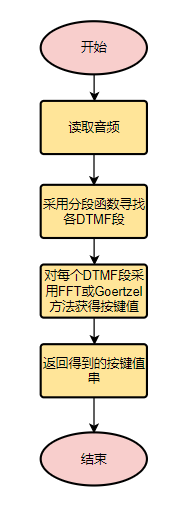
\includegraphics[scale=0.8]{assets/6.png}}

\section{结果与分析}

\subsection{DTMF信号产生}
采用时长t=0.2s,分别键入不同的按键,得到的结果图像如下:

按键值为5时,输出DTMF信号为:

\centerline{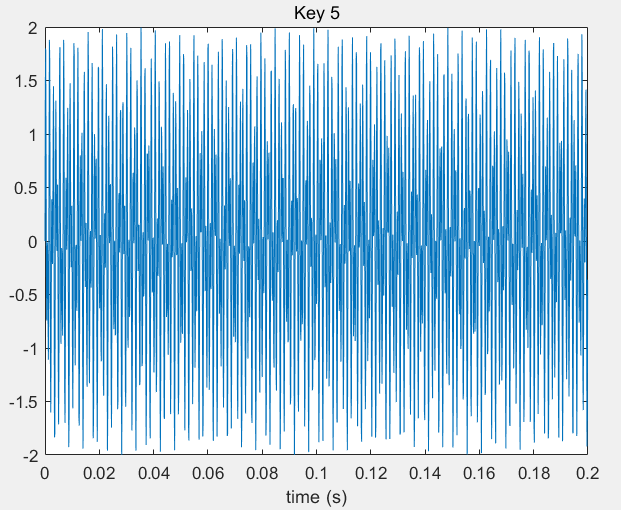
\includegraphics[scale=0.8]{assets/8.png}}

按键值为B时,输出DTMF信号为:

\centerline{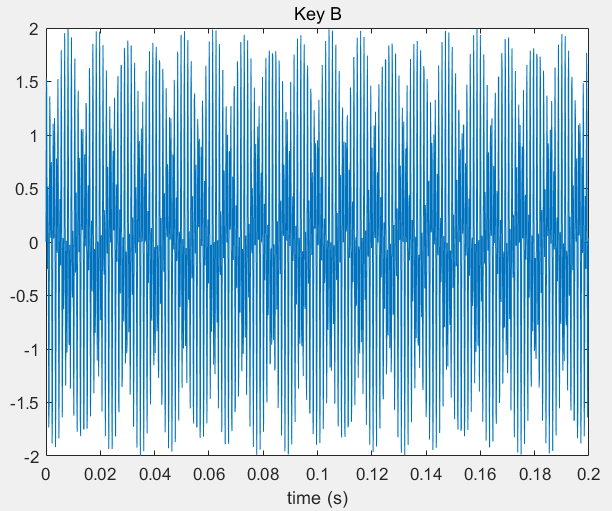
\includegraphics[scale=0.8]{assets/9.png}}

\subsection{DTMF信号检测识别}

\subsubsection{FFT方法}

\centerline{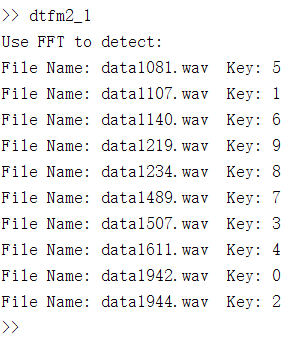
\includegraphics[scale=1.0]{assets/10.png}}

\subsubsection{Goertzel算法}

\centerline{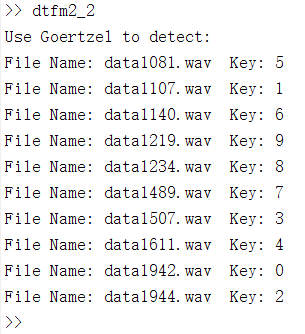
\includegraphics[scale=1.0]{assets/11.png}}

可以看到两种方法得到的结果是一致的。

\subsection{长音频检测}

下图为分段函数探测各DTMF段的结果(其中,红色表示DTMF段的开始,蓝色表示DTMF段的结束):

\centerline{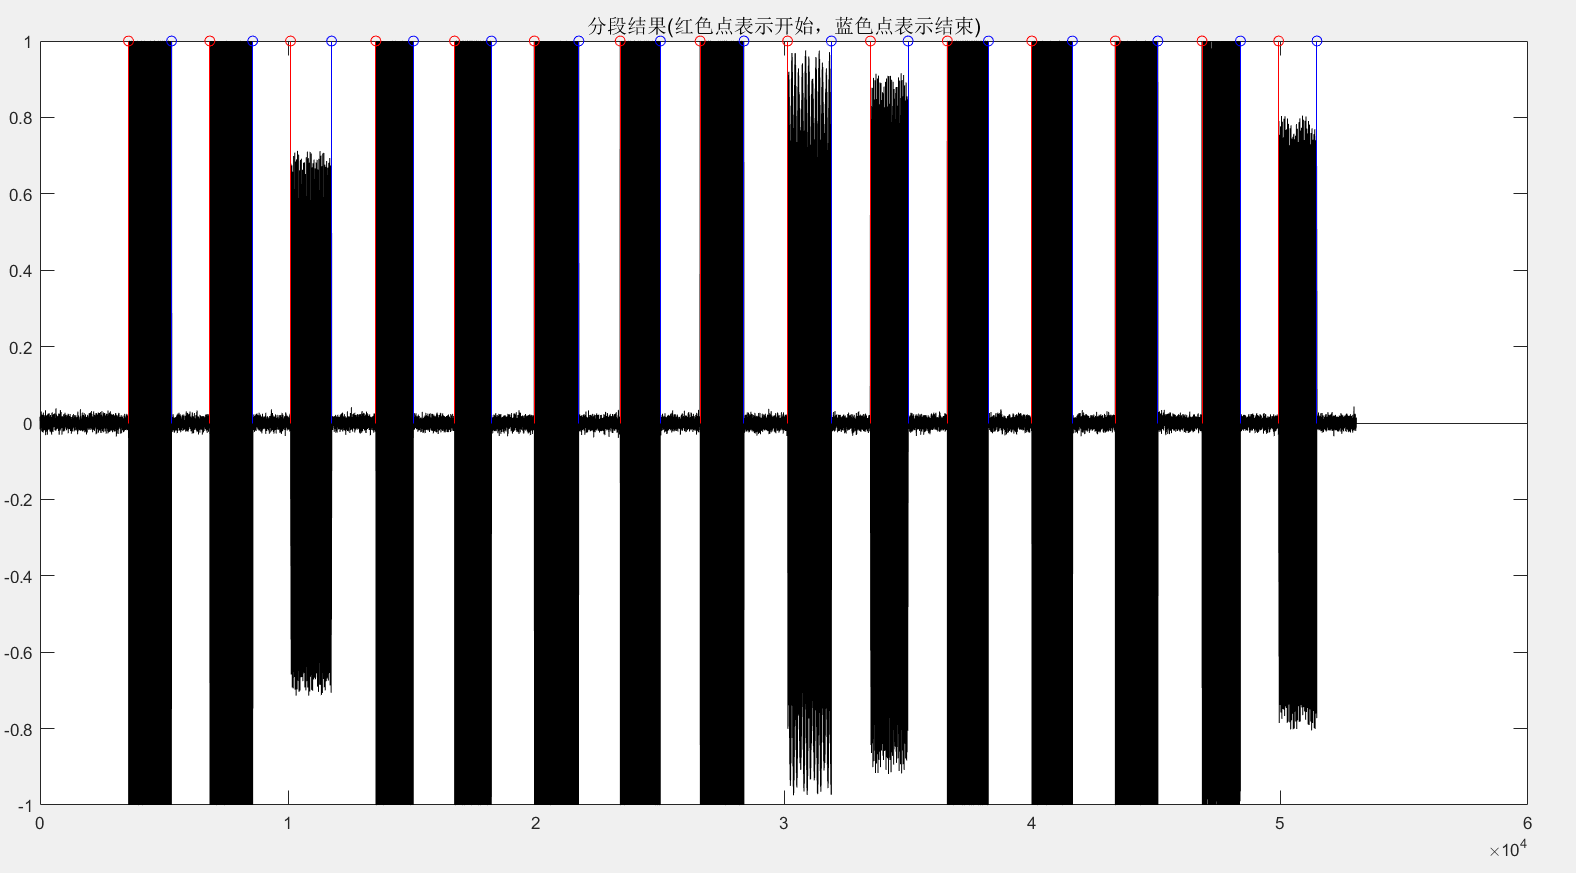
\includegraphics[scale=0.45]{assets/12.png}}

下图为采用两种方法对长音频各DTMF段检测结果所得的按键值串(X表示错误):

\centerline{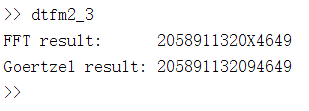
\includegraphics[scale=1]{assets/13.png}}

可以看到,除去倒数第5处外,两种方法得到的结果是一致的。

在FFT方法的检测中,将此处识别为错误,经过我进一步的检查,我发现,此处的音频可能本身就存在错误。

将这一段音频信号做FFT的结果取出来,如下图所示:

\centerline{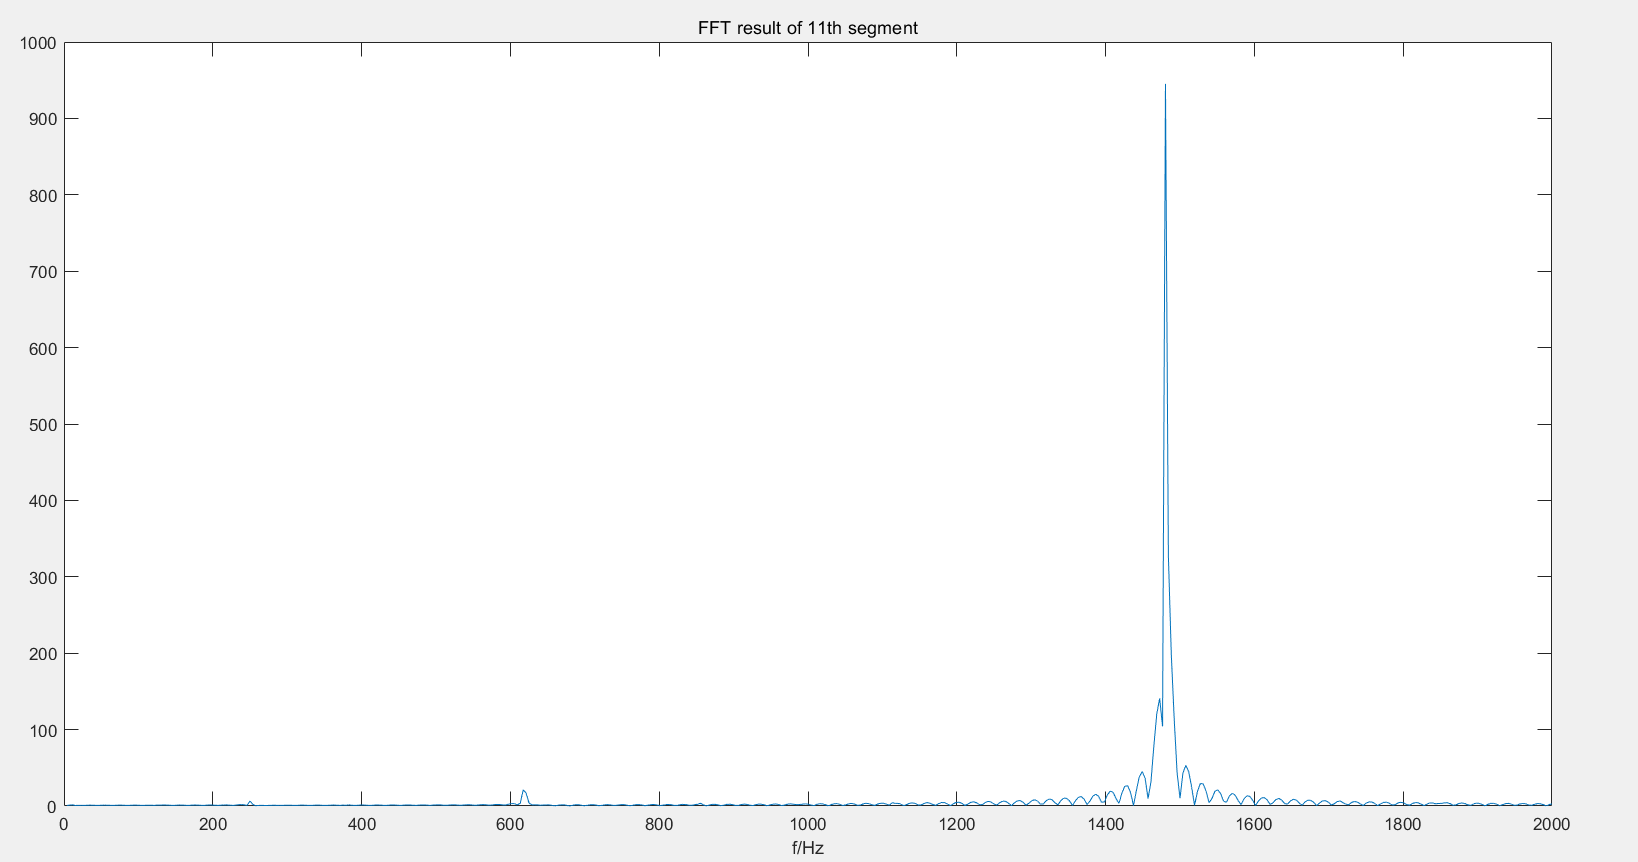
\includegraphics[scale=0.45]{assets/14.png}}

可以看到,只在1477Hz前后处,有一个单峰,其他频率点基本上都很小,610Hz处也有一个非常小的峰,但是此处并非有效频率,由此可以认为这段音频信号包含不正确的频率组合。

\subsection{两种方法识别性能对比分析}

主要从计算复杂度和识别鲁棒性这两个角度来进行对比分析。

\subsubsection{计算复杂度}

\begin{enumerate}
    \item 基于FFT的识别算法
    
    对于一个长度为N的片段(忽略补零),采用基2-FFT算法的时间复杂度为$O(N\log N)$,具体而言需要$2N\log_2 N$次实乘和$3N\log_2 N$次实加。
    
    执行完DFT后需要寻找峰值,该操作的时间复杂度为$O(N)$。
    
    故而总体的时间复杂度为$O(N\log N)$。
    
    \item 基于Goertzel的识别算法
    
    对于一个长度为N的片段,由于只关心8个频点,时间复杂度为$O(N)$,而此后只需在8个频点中去寻找低频和高频区的最大值,该部分为常数时间复杂度,故而总体的时间复杂度为$O(N)$。
    
\end{enumerate}

由此可见,在计算时间复杂度上,基于Goertzel的识别算法是要明显优于基于FFT的识别算法的。并且实际在Matlab中运行并计时也可以看到基于Goertzel的识别算法是要明显快于基于FFT的识别算法的。

\subsubsection{鲁棒性}

根据之前的长音频检测过程和结果,我们可以看到,对于其中的一个错误的DTMF段,FFT轻松的发现了错误存在,而Goertzel则由于算法自身设计的原因,依然给出了一个结果。由此可见,基于FFT的识别方法虽然计算复杂度较高,但是其可以更好的应对各种错误情况。

\section{总结}

本次课程设计中,我除了进一步熟练使用FFT这一工具进行信号分析之外,还学习了Goertzel这一种全新的算法。这种算法可以说是利用了更多的条件约束来达到更低的时间复杂度。对于长音频信号的分析中比较核心的分割问题,我也尝试了好几种方法,最后根据长音频信号的特点选择了现在所使用的方法,最后实现效果很好。这一次课程设计过程中,我除了巩固了已经学习的知识之外,也更加深切地感悟到了DSP理论应用于实际时的强大威力,可以说是收获满满。

\clearpage
\section{文件清单}

\begin{table}[h]
    \centering
    \begin{tabular}{ll}
        \toprule
        文件名称         & 说明                       \\
        \midrule
        dtfm2\_1.m           & 采用FFT进行10个文件检测的主程序 \\
        dtfm2\_2.m           & 采用Goertzel进行10个文件检测的主程序 \\
        dtfm2\_3.m           & 采用两种方法检测识别长音频文件的主程序 \\
        dtmf1.m             & 产生DTMF信号的的主程序 \\
        find\_key\_fft.m      & 根据音频信号采用FFT检测对应按键值的函数 \\
        find\_key\_goertzel.m & 根据音频信号采用Goertzel检测对应按键值的函数 \\
        generate\_dtmf.m     & 产生DTMF信号的函数 \\
        \bottomrule
    \end{tabular}
\end{table}

备注:需将存放音频数据的\textit{附件1}和\textit{附件2}这两个文件夹放置在此根目录中方可运行

\end{document}
